\documentclass{beamer}
\mode<presentation>
\usetheme{CambridgeUS}
\usepackage[russian]{babel}
\usepackage[utf8]{inputenc}
\usepackage[T2A]{fontenc}
\usepackage{sansmathaccent}

\usepackage{verbatim}
\usepackage{alltt}

\pdfmapfile{+sansmathaccent.map}
\title[Artifical Intelligence]{Нейронные сети}
\author{Наумов Д.А., доц. каф. КТ}
\date[11.02.2019] {Экспертные системы и искусственный интеллект, 2019}

\begin{document}

%ТИТУЛЬНЫЙ СЛАЙД
\begin{frame}
  \titlepage
\end{frame}
  
%СОДЕРЖАНИЕ ЛЕКЦИИ
\begin{frame}
  \frametitle{Содержание лекции}
  \tableofcontents  
\end{frame}

%\section{Математические основы нейронных сетей}
%\subsection{Представление данных для нейронных сетей}
%\subsection{Операции с тензорами}

\section{Тренировка алгоритмов машинного обучения для задач классификации}

\begin{frame}[t]{План изучения темы}
\begin{enumerate}
\item изучение первых алгоритмических методов классификации данных - персептрон и адаптивный линейными нейрон; 
\item пошаговая реализация персептрона на языке Python и его тренировки для решения;
\item задача классификации различных видов цветков из набора данных Ирисов Фишера;
\item азы оптимизации с использованием адаптивных линейных нейронов;
\item использование библиотек pandas, NumPy и matplotlib для чтения, обработки
и визуализации данных;
\item реализация алгоритмов линейной классификации на Python.
\end{enumerate}
\end{frame}

\subsection{Краткий обзор истории}
\begin{frame}[t]{Модель нейрона}
\begin{figure}[h]
\centering
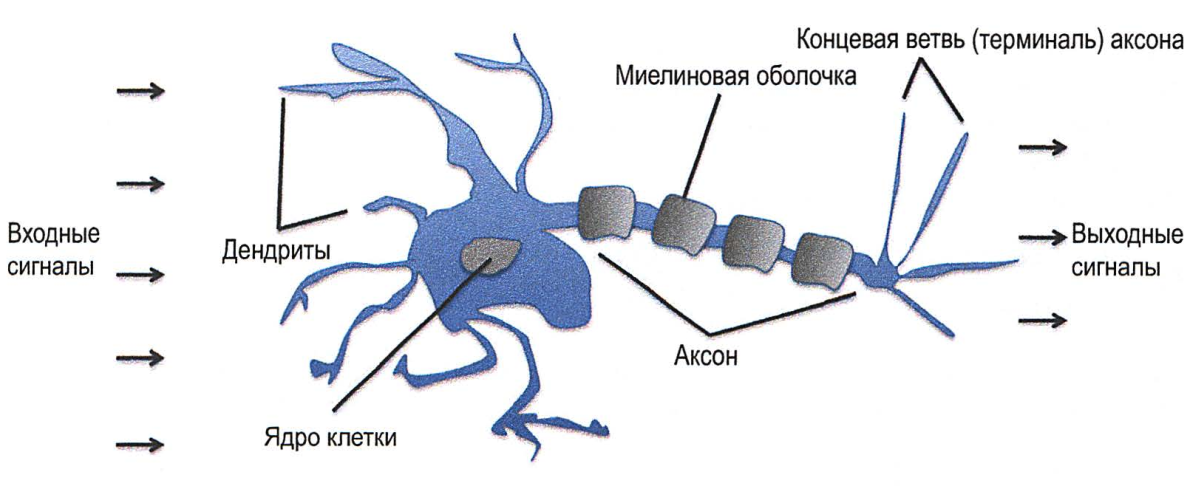
\includegraphics[scale=0.3]{images/lec03-pic01.png}
\end{figure}
\begin{enumerate}
\item У. Маккалок и У. Питтс, «Логическое исчисление идей, относящихся к нервной активности», Bulletin of Mathematical Biophysics (Бюллетень математической биофизики), 5 (4):115-133, 1943);
\item Ф. Розенблатт, .-.Лерсептрон, воспринимающий и распознающий автомат», Coгnell
Aeronautical Laboratoгy (Лаборатория аэронавтики Корнелльского университета),
1957).
\end{enumerate}
\end{frame}

\begin{frame}[t]{Задача бинарной классификации}
\begin{itemize}
\item задаются \textbf{два класса}: 1 (положительный класс), -1 (отрицательный класс);
\item рассчитывается \textbf{чистый вход} - линейная комбинация весов и входных значений $z=w_1\cdot x_1+...+w_m\cdot x_m$;
\end{itemize}
\begin{figure}[h]
\centering
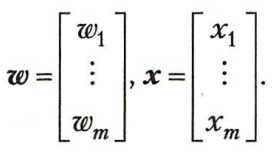
\includegraphics[scale=0.5]{images/lec03-pic02.png}
\end{figure}
\begin{itemize}
\item определяется передаточная функцию (функция активации) $\phi(z)$;
\item в алгоритме персептрона функция активации - это простая ступенчатая функция Хевисайда;
\end{itemize}
\begin{figure}[h]
\centering
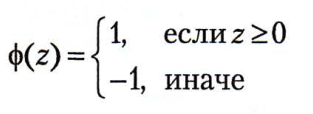
\includegraphics[scale=0.4]{images/lec03-pic03.png}
\end{figure}
\end{frame}

\begin{frame}[t]
\begin{itemize}
\item активация отдельно взятого образца $x^{(i)}$, т. е. выход из $\phi(z)$, превышает заданный порог, то мы распознаем класс 1, в противном случае - класс -1;
\item порог учитывается так: $w_0 = -\theta, x_0 = -1$;
\end{itemize}
\begin{figure}[h]
\centering
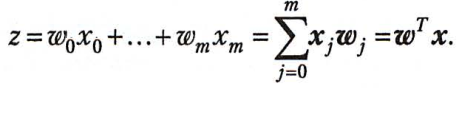
\includegraphics[scale=0.4]{images/lec03-pic04.png}
\end{figure}
\begin{figure}[h]
\centering
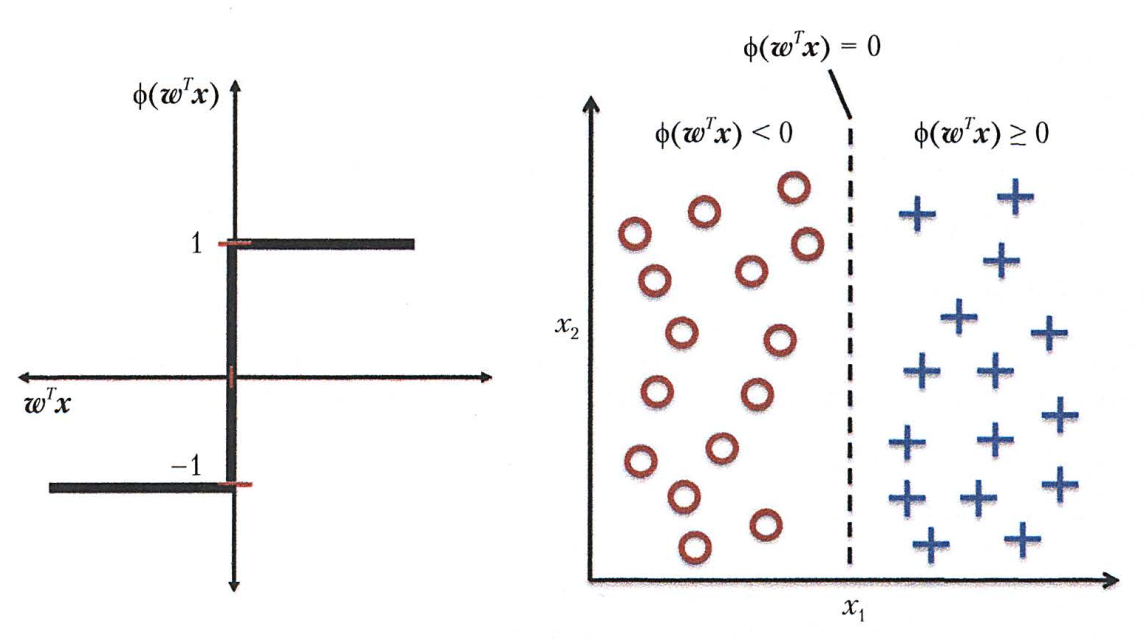
\includegraphics[scale=0.25]{images/lec03-pic05.png}
\end{figure}
\end{frame}

\begin{frame}[t]
Идея, лежащая в основе нейрона MCP и персептронной модели Розенблатта с порогом:
\begin{enumerate}
\item инициализировать веса нулями либо малыми случайными числами;
\item для каждого тренировочного образца $x^{(i)}$ выполнить следующие шаги:
\begin{itemize}
\item вычислить выходное значение $\hat{y}$;
\item обновить веса.
\end{itemize}
\end{enumerate}
\textbf{Выходное значение} - метка класса, идентифицированная единичной
ступенчатой функцией.
\[\omega_j := \omega_j + \Delta\omega_j\]
Значение $\Delta\dot\omega_j$ вычисляется правилом обучения персептрона:
\[\Delta\omega_j := \eta(y^{(i)} - \hat{y}^{(i)})x^{(i)}_j \]
\begin{itemize}
\item $\eta$ - темп обучения (константа 0.0..1.0);
\item $y^{(i)}$ - истинная метка класса i-го тренировочного образца;
\item $\hat{y}^{(i)}$ - идентифицированная метка класса. 
\end{itemize}
\end{frame}

\begin{frame}[t]
Персептрон правильно распознает метку класса, веса остаются неизменными:
\begin{figure}[h]
\centering
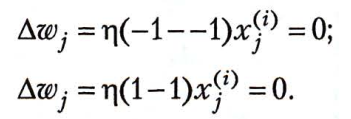
\includegraphics[scale=0.5]{images/lec03-pic06.png}
\end{figure}
В случае неправильного распознавания веса продвигаются в направлении
соответственно положительного или отрицательного целевого класса:
\begin{figure}[h]
\centering
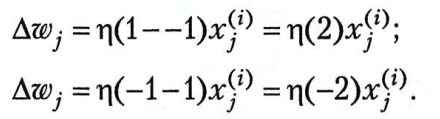
\includegraphics[scale=0.5]{images/lec03-pic07.png}
\end{figure}
\end{frame}

\begin{frame}[t]
Замечания о сходимости:
\begin{enumerate}
\item сходимость персептрона гарантируется, только если эти два класса линейно разделимы и темп обучения достаточно небольшой. 
\item если эти два класса не могут быть разделены линейной границей решения, необходимо установить максимальное число проходов по тренировочному набору данных (эпох) и/или порог на допустимое число случаев ошибочной классификации, иначе обновление весов будет продолжаться бесконечно.
\end{enumerate}
\begin{figure}[h]
\centering
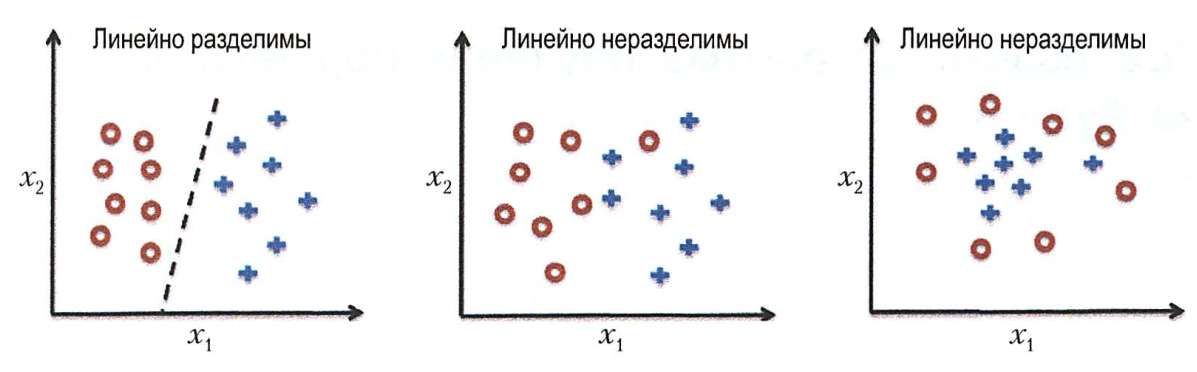
\includegraphics[scale=0.35]{images/lec03-pic08.png}
\end{figure}
\end{frame}

\begin{frame}[t]{Схема MCP}
\begin{figure}[h]
\centering
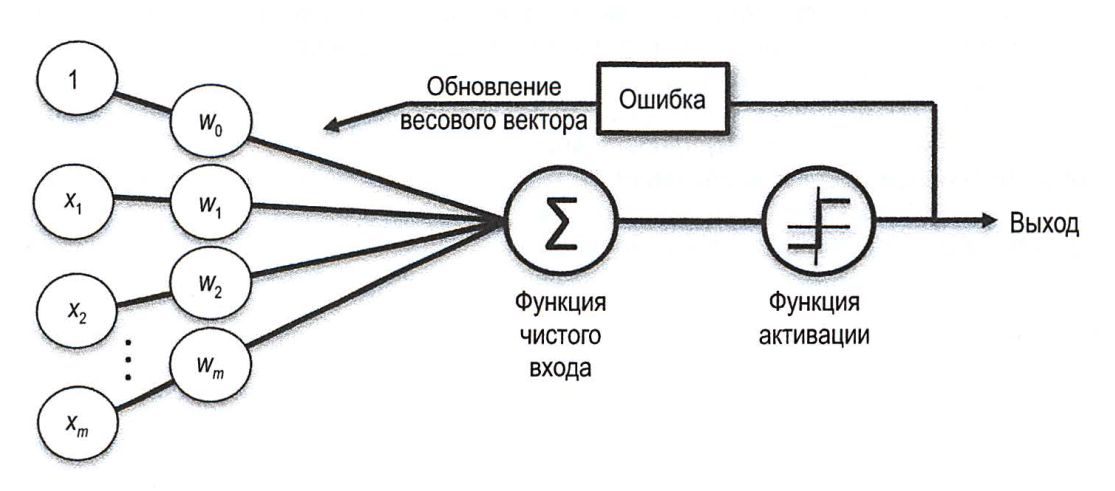
\includegraphics[scale=0.4]{images/lec03-pic09.png}
\end{figure}
\end{frame}

\subsection{Реализация персептрона на Python}
\begin{frame}[t]
\begin{figure}[h]
\centering
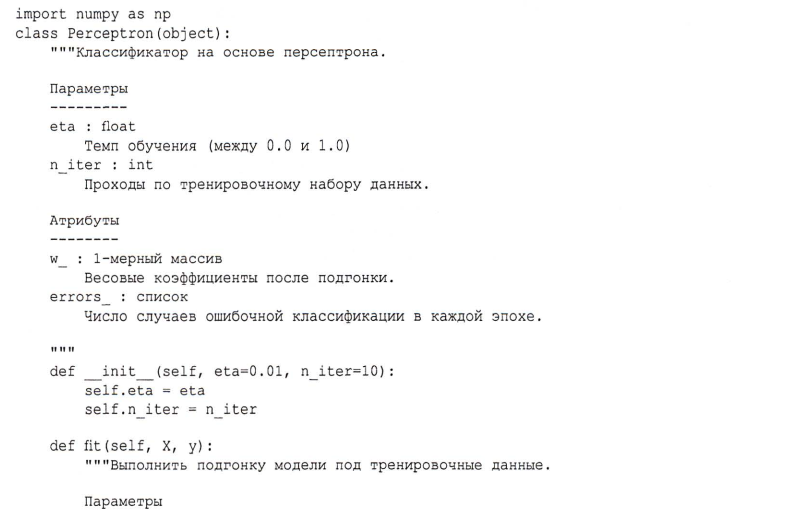
\includegraphics[scale=0.5]{images/lec03-pic10.png}
\end{figure}
\end{frame}

\begin{frame}[t]
\begin{figure}[h]
\centering
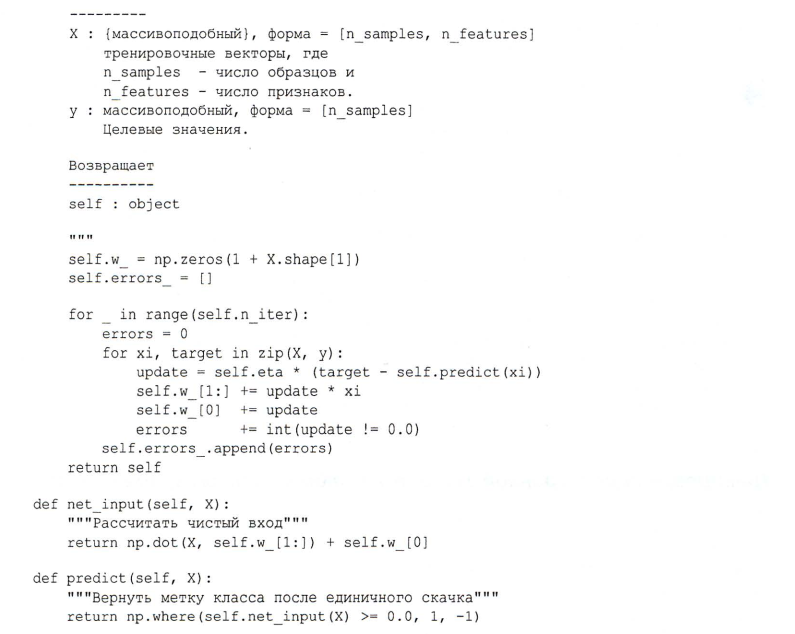
\includegraphics[scale=0.5]{images/lec03-pic11.png}
\end{figure}
\end{frame}

\subsection{Реализация алгоритма обучения и тренировка персептрона}
\begin{frame}[t]
Тренировка персептронной модели на наборе данных цветков ириса
\begin{enumerate}
\item загрузим из набора данных ирисов два класса цветков: ирис щетинистый (Iri.s setosa) и ирис разноцветный (Iri.sversicolor). 
\item в целях визуализации рассмотрим только два признака - длина
чашелистика (sepal leпgth) и длина лепестка (petal leпgth).
\end{enumerate}
\begin{figure}[h]
\centering
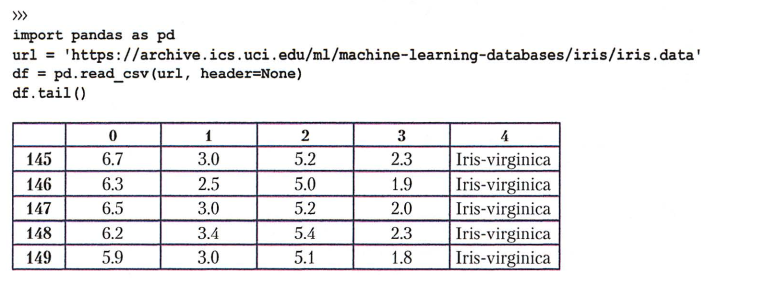
\includegraphics[scale=0.5]{images/lec03-pic12.png}
\end{figure}
\end{frame}

\begin{frame}[t]
\begin{figure}[h]
\centering
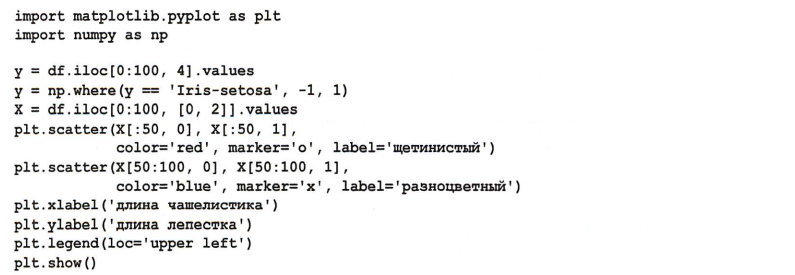
\includegraphics[scale=0.5]{images/lec03-pic13.png}
\end{figure}
\begin{figure}[h]
\centering
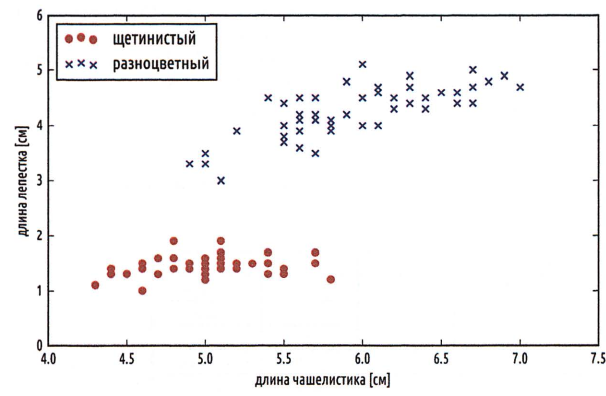
\includegraphics[scale=0.4]{images/lec03-pic14.png}
\end{figure}
\end{frame}

\begin{frame}[t]
\begin{figure}[h]
\centering
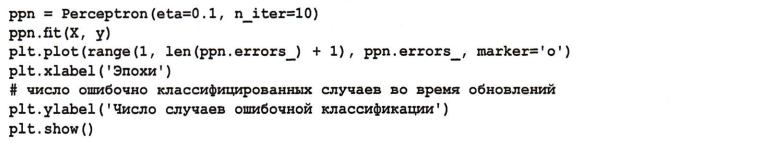
\includegraphics[scale=0.5]{images/lec03-pic15.png}
\end{figure}
\begin{figure}[h]
\centering
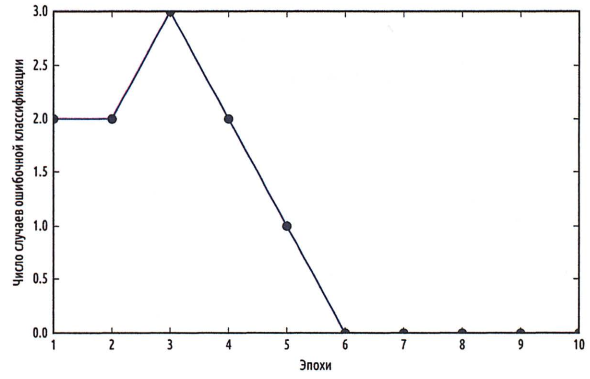
\includegraphics[scale=0.5]{images/lec03-pic16.png}
\end{figure}
\end{frame}

\begin{frame}[t]
\begin{figure}[h]
\centering
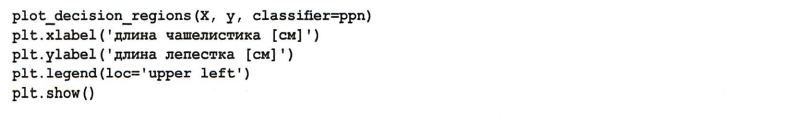
\includegraphics[scale=0.5]{images/lec03-pic17.png}
\end{figure}
\begin{figure}[h]
\centering
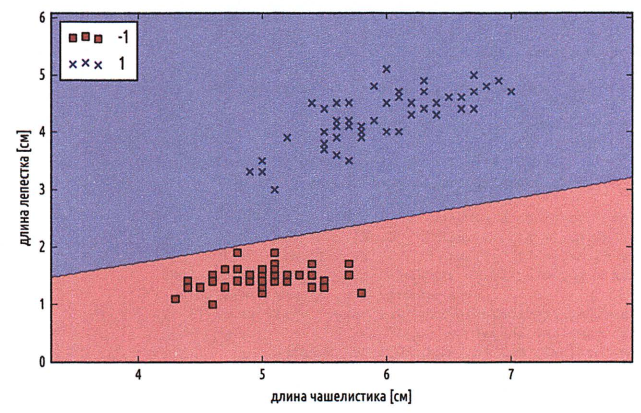
\includegraphics[scale=0.5]{images/lec03-pic18.png}
\end{figure}
\end{frame}

\subsection{Аддитивные линейные нейроны и сходимость обучения}

\begin{frame}[t]
\textbf{ADALINE} - ADAptive LInear NEuron, адаптивный линейный нейрон.
\begin{itemize}
\item для обновления весов используется линейная функция активации $\phi(\omega^T x) = \omega^Tx$,
а не единичная ступенчатая, как в персептроне;
\item с целью распознавания меток классов используется квантизатор, аналогичный встречавшейся ранее единичной ступенчатой функции.
\end{itemize}
\begin{figure}[h]
\centering
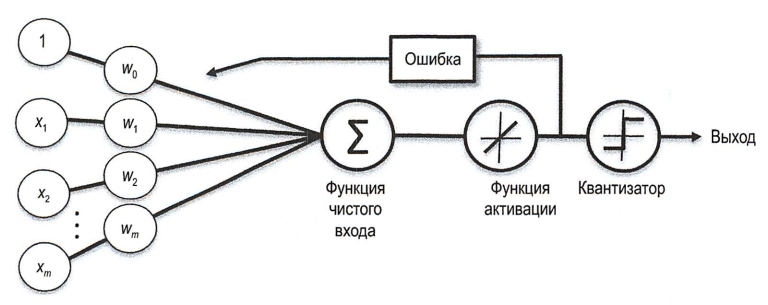
\includegraphics[scale=0.4]{images/lec03-pic19.png}
\end{figure}
Б. Видроу и др., Adaptive «Adalineineuгon using chemical «me mistoгsi- («Адаптивный нейрон "Adaliпe" с использованием химических "мемисторов"~- ). Numbeг Technical Repoгt Stanfoгd Electгon . Labs, Стэнфорд, Калифорния, октябрь 1960)
\end{frame}

\begin{frame}[t]
\textit{Ключевая составляющая алгоритмов машинного обучения с учителем}: задание целевой функции, которая подлежит оптимизации во время процесса обучения.
\begin{figure}[h]
\centering
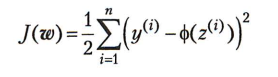
\includegraphics[scale=0.6]{images/lec03-pic20.png}
\end{figure}
Применяемый алгоритм оптимизации - \textbf{алгоритм градиентного спуска} для нахождения весов, которые минимизируют функцию стоимости.
\begin{figure}[h]
\centering
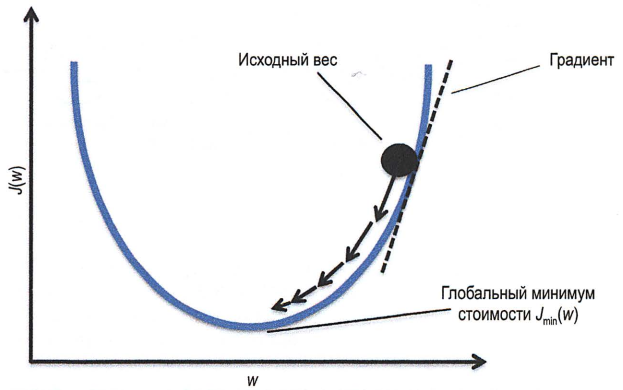
\includegraphics[scale=0.4]{images/lec03-pic21.png}
\end{figure}
\end{frame}

\begin{frame}[t]
Обновление веса на основе градиентного спуска путем выполнения
шага в противоположную сторону от градиента функции стоимости
\begin{figure}[h]
\centering
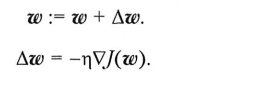
\includegraphics[scale=0.75]{images/lec03-pic22.png}
\end{figure}
Для расчета градиента функции стоимости нужно вычислить частную производную функции стоимости относительно каждого веса: 
\begin{figure}[h]
\centering
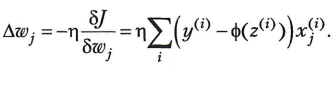
\includegraphics[scale=0.75]{images/lec03-pic23.png}
\end{figure}
\begin{itemize}
\item значение $\phi(z^{(i)})$ - вещественное число, а не целочисленная метка класса;
\item обновление веса вычисляется на основе всех образцов в тренировочном наборе, и поэтому такой подход называется "пакетным" (batch) градиентным спуском.
\end{itemize}
\end{frame}

\subsection{Реализация адаптивного линейного нейрона}
\begin{frame}[t]
\begin{figure}[h]
\centering
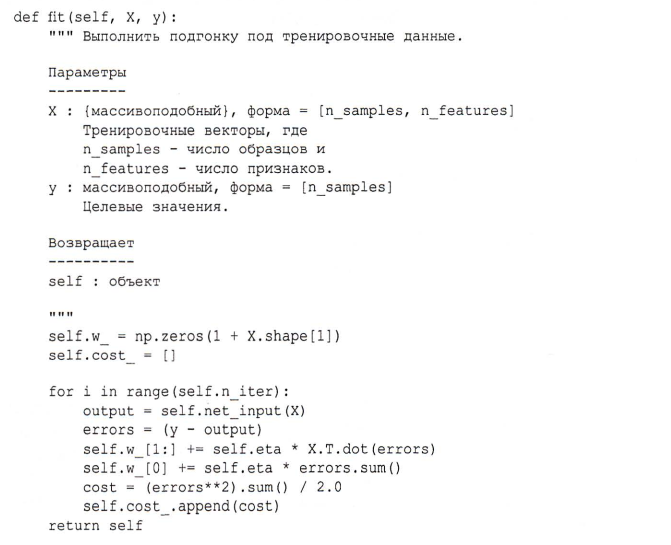
\includegraphics[scale=0.6]{images/lec03-pic24.png}
\end{figure}
\end{frame}

\begin{frame}[t]{График стоимости в зависимости от числа эпох}
\begin{figure}[h]
\centering
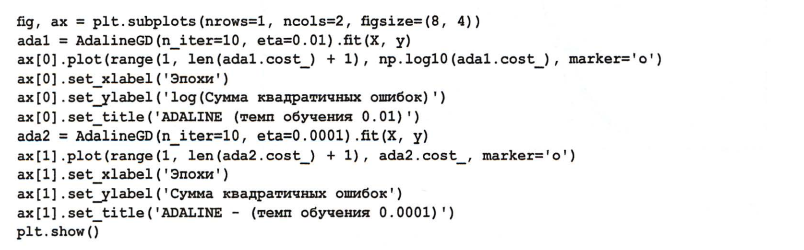
\includegraphics[scale=0.4]{images/lec03-pic25.png}
\end{figure}
\begin{figure}[h]
\centering
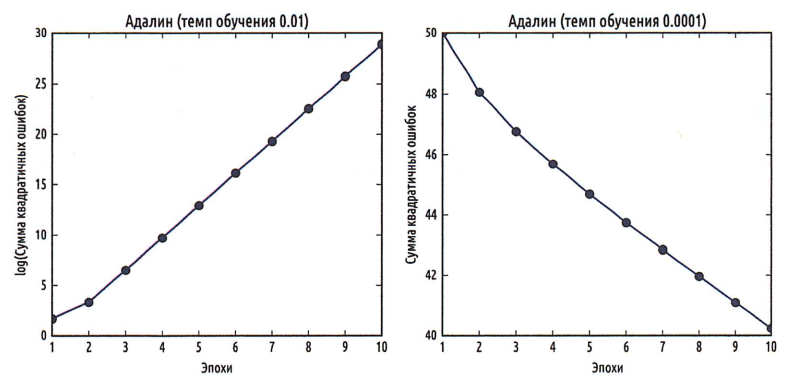
\includegraphics[scale=0.4]{images/lec03-pic26.png}
\end{figure}
\end{frame}

\begin{frame}[t]
\begin{figure}[h]
\centering
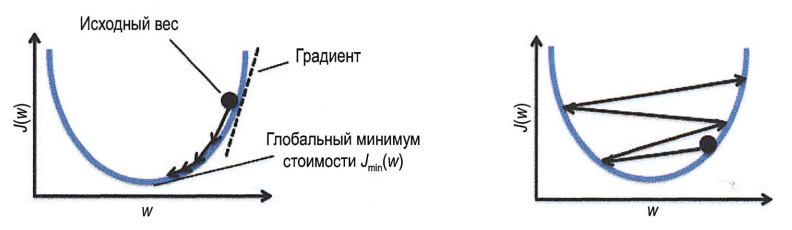
\includegraphics[scale=0.6]{images/lec03-pic27.png}
\end{figure}
Алгоритм градиентного спуска можно улучшить, выполнив предварительное масштабирование признаков. 
\begin{figure}[h]
\centering
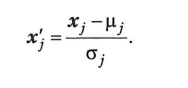
\includegraphics[scale=0.6]{images/lec03-pic28.png}
\end{figure}
\begin{figure}[h]
\centering
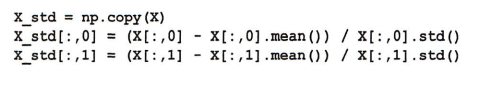
\includegraphics[scale=0.6]{images/lec03-pic29.png}
\end{figure}
\end{frame}

\begin{frame}[t]
\begin{figure}[h]
\centering
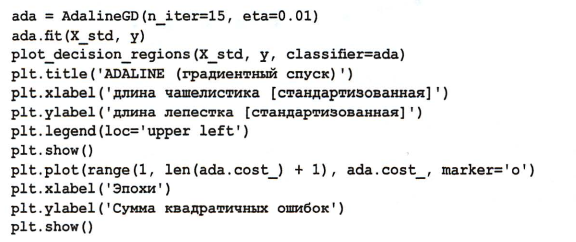
\includegraphics[scale=0.6]{images/lec03-pic30.png}
\end{figure}
\begin{figure}[h]
\centering
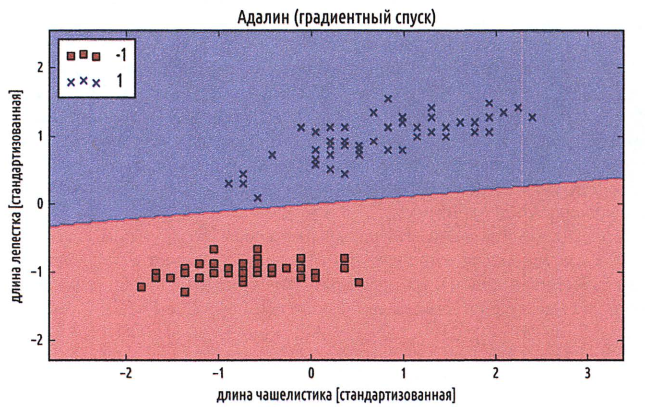
\includegraphics[scale=0.4]{images/lec03-pic31.png}
\end{figure}
\end{frame}

\begin{frame}[t]
\begin{figure}[h]
\centering
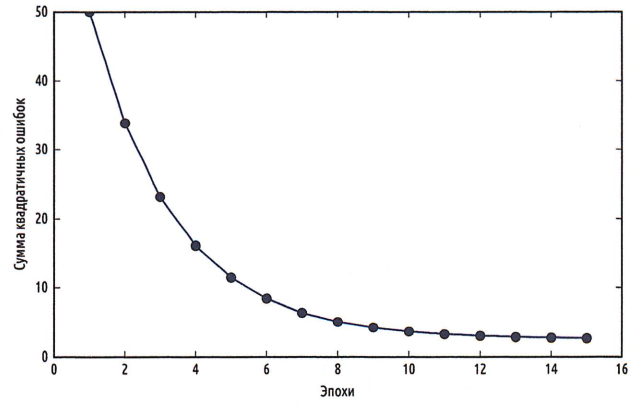
\includegraphics[scale=0.6]{images/lec03-pic32.png}
\end{figure}
\begin{itemize}
\item ADALINE сходится после тренировки на стандартизированных признаках с темпом обучения Т = 0.01; 
\item сумма квадратичных ошибок (SSE) остается ненулевой даже при том, что все
образцы были классифицированы правильно.
\end{itemize}
\end{frame}

\subsection{Оптимизация на основе стохастического градиентного спуска}

\begin{frame}[t]
Для большых наборов данных выполнение пакетного градиентного спуска может быть
в вычислительном плане довольно дорогостоящим, поскольку необходимо выполнять переоценку всего тренировочного набора данных каждый раз, когда мы делаем
один шаг к глобальному минимуму.
\begin{block}{Стохастический градиентный спуск}
вместо обновления весов, основываясь на сумме накопленных ошибок по всем образцам, обновляет веса инкрементно по каждому тренировочному образцу:
\begin{figure}[h]
\centering
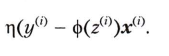
\includegraphics[scale=0.6]{images/lec03-pic33.png}
\end{figure}
\begin{itemize}
\item намного быстрее достигает сходимости;
\item лучше выходит из мелких локальных минимумов;
\item важно перемешивать тренировочный набор в каждой эпохе;
\item возможность тренировки "на лету".
\end{itemize}
\end{block}
\end{frame}

\begin{frame}[t]{Корректировки алгоритма ADALINE}
\begin{itemize}
\item в методе fit будут обновляться веса после каждого тренировочного образца;
\item реализован дополнительный метод частичной подгонки partial\_fit, который повторно не инициализирует веса, чтобы учесть динамическое обучение;
\item для провреки, что алгоритм сходился после тренировки, вычисляется стоимость как усредненную стоимость тренировочных образцов в каждой эпохе;
\item опцию shuffle - перемешивание тренировочных данных перед каждой эпохой для предотвращения зацикливания во время оптимизации функции стоимости.
\end{itemize}
\end{frame}

\begin{frame}[t]
\begin{figure}[h]
\centering
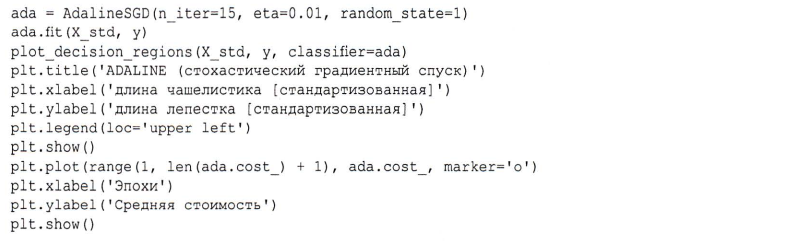
\includegraphics[scale=0.5]{images/lec03-pic34.png}
\end{figure}
\begin{figure}[h]
\centering
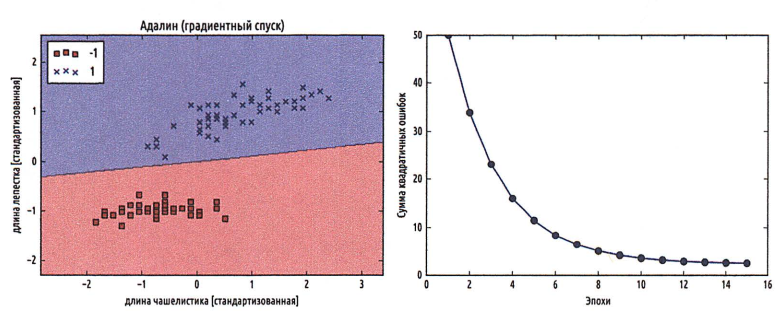
\includegraphics[scale=0.5]{images/lec03-pic35.png}
\end{figure}
\end{frame}

\end{document}
